\documentclass[]{scrartcl}

\usepackage[ngerman]{babel}
\usepackage[utf8]{inputenc}

\usepackage{calligra} % font
\usepackage{hyperref} % URLs, links
\usepackage{lscape} % landscape mode
\usepackage{tabularx} % tables

\usepackage{tabularx} % tables
\usepackage{xargs} % multiple parameters

\newcolumntype{Y}{>{\centering\arraybackslash}X} % same as 'X' but centered

\newcommandx{\dndtextbox}[2][1=\linewidth]{
	{
		\setlength{\fboxsep}{1em}
		\fbox{
			\parbox{#1}{
				#2
			}
		}
	}
}

\newcommandx{\dndspell}[8][1=-, 2=-, 3=-, 4=-, 5=-, 6=-, 7=~, 8=~]{
	\begin{tabularx}{\linewidth}{X}
		{\Large \bfseries{#1}}\\
		~\\
		{\small \textit{#2}}\\
		~\\
		{\footnotesize {\bfseries Zeitaufwand:} #3}\\
		{\footnotesize {\bfseries Reichweite:} #4}\\
		{\footnotesize {\bfseries Komponenten:} #5}\\
		{\footnotesize {\bfseries Wirkungsdauer:} #6}\\
		~\\
		{\scriptsize #7}\\
		{\scriptsize #8}
	\end{tabularx}
}

\newcommandx{\dndmonsterheader}[5][1=-, 2=-, 3=-, 4=-, 5=-]{
	{\Large \bfseries{#1}}\\
	{\small \textit{#2}}\\
	~\\
	{\footnotesize {\bfseries Rüstungsklasse:} #3}\\
	{\footnotesize {\bfseries Trefferpunkte:} #4}\\
	{\footnotesize {\bfseries Bewegungsrate:} #5}\\
	~\\
}

\newcommandx{\dndmonsterattributes}[6][1=-, 2=-, 3=-, 4=-, 5=-, 6=-]{
	\begin{tabularx}{\linewidth}{YYYYYY}
		{\small {\bfseries STR}} &
		{\small {\bfseries GES}} &
		{\small {\bfseries KON}} &
		{\small {\bfseries INT}} &
		{\small {\bfseries WEI}} &
		{\small {\bfseries CHA}}\\
		
		{\small #1} &
		{\small #2} &
		{\small #3} &
		{\small #4} &
		{\small #5} &
		{\small #6}
	\end{tabularx}
	~\\
}

\newcommandx{\dndmonsterinfo}[4][1=-, 2=-, 3=-, 4=-]{
	{\footnotesize {\bfseries Fertigkeiten:} #1}\\
	{\footnotesize {\bfseries Sinne:} #2}\\
	{\footnotesize {\bfseries Sprachen:} #3}\\
	{\footnotesize {\bfseries Herausforderungsgrad:} #4}\\
	~\\
}

\newcommandx{\dndmonsterfeature}[2]{
	{\footnotesize {\bfseries #1:} #2}\\
	~\\
}

\newcommandx{\dndattack}[5]{
	\textit{#1:} #2 auf Treffer, Reichweite #3, #4. \textit{Treffer:} #5
}


\titlehead{\centering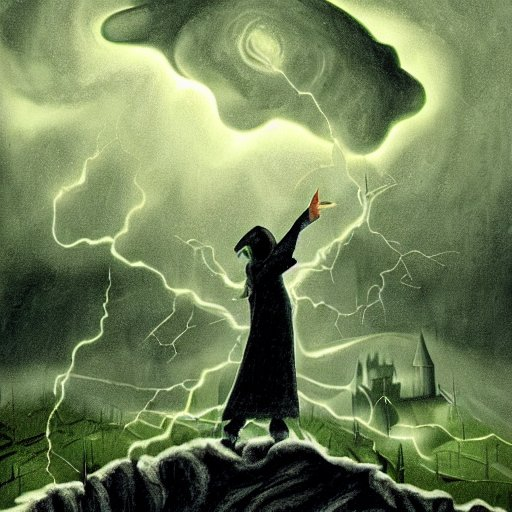
\includegraphics[width=0.5\linewidth]{cover}}
\title{Nathair's Fluch}
\author{Moritz Fink}

\begin{document}

\maketitle

\begin{abstract}
\textit{
Diese Dungeons \& Dragons Kampagne für 2-4 Charaktere (1. Stufe) wurde inspiriert von J.K. Rowling und David Ng (vgl. \url{https://popperfont.files.wordpress.com/2016/12/hpddcampaign1.pdf}). Dieses Skript ist dabei ausschließlich für den Spielleiter vorgesehen.\\
}

Als eines Tages ein mysteriöser Brief auf dem Tisch liegt, müssen sich normale Muggel als Zauberer beweisen, um Luna's Zauberstab sicher nach Hogwarts zu bringen. Dort angekommen, fällt dieser jedoch in die Hände des bösen Zauberers Nathair, welcher Hogwarts in eine Ruine verwandelt. Können sich die mutigen Abenteurer in dieser harten Prüfung beweisen oder ist das das Ende der einst so prunkvollen Zauberschule?
\end{abstract}

\newpage

\tableofcontents

\newpage

\section{Auftakt (30min)}

Das Abenteuer beginnt mit einem Brief, welcher die Spieler zunächst in die Kampagne einführt und ihre Charaktere erstellen lässt.

\subsection{Ein mysteriöser Brief}

Die Spieler versammeln sich am Tisch und finden dort Luna's Zauberstab, einen Brief und jeweils einen Teebeutel vor. Der Spielleiter sollte vorerst in keinster Weise eingreifen, damit die Spieler den Brief lesen und entsprechende Aktionen ableiten können. Aus dem Inhalt sollte relativ schnell ersichtlich sein, dass sich die Spieler zuerst Tee machen sollen. Die Zeit bis dieser trinkbar ist sollte mit der Suche nach einem geeigneten Zauberstabersatz und der Charaktererstellung gefüllt werden.

\newpage

{\calligra \large
	
Liebe Muggel,\\

uns bleibt nur wenig Zeit, die Situation zu erklären. Also werden wir uns kurzfassen.\\

Der Zauberstab, welchen ihr besitzt, ist mit äußerster Vorsicht zu behandeln, denn es handelt sich in Wirklichkeit um den Zauberstab unserer Mutter. Große und mächtige Taten wurden damit schon vollführt!\\

Doch als er zu einer Gefahr für die freie Welt der Hexen und Zauberer wurde, haben wir ihn (schlauerweise) als Spielzeug getarnt in einem Muggelgeschäft versteckt, damit er vor den Augen dunkler Mächte verschlossen bleibt. Bedauerlicherweise können wir nicht mehr für eure Sicherheit garantieren, da Nathair’s Schüler herausgefunden haben, wo sich der Zauberstab befindet.\\

Somit tragt ihr nun die Bürde, ihn sicher nach Hogwarts zu bringen und an eine gewisse Mrs. Weasley-Granger zu übergeben.\\

Um euch bei dieser Aufgabe zu helfen, haben wir dem Brief Teebeutel beigelegt. Sucht euch jeweils einen Zauberstabersatz (etwas Zauberstab-artiges) und haltet diesen fest in eurer Hand, während ihr euren Tee genießt. Sobald jeder von euch getrunken hat, fungiert der (echte) Zauberstab als Portschlüssel. Stellt sicher, dass ihr ihn alle gleichzeitig berührt und alles Wichtige mitnehmt!\\

Sobald ihr angekommen seid, steigt \underline{zügig} ein und achtet darauf, dass ihr nicht verfolgt werdet. Findet den Ort an dem \underline{nur ein Stück pro Person} erlaubt ist. Dort befindet sich der \underline{Schlüssel} nach Hogwarts.\\

Beeilt euch, denn es gilt keine Sekunde zu verlieren!\\

~\\

Hochachtungsvoll\\
Lorcan \& Lysander
}

\newpage

\subsection{Charakterbögen}

Der Spielleiter händigt jeweils einen D\&D Charakterbogen an jeden Spieler aus und führt durch die Charaktererstellung. Diese richtet sich im Großen und Ganzen nach dem D\&D 5e Regelwerk, allerdings mit folgenden Modifikationen:
\begin{itemize}
	\item Jeder Spieler spielt sich selbst
	\item Klasse = Magier
	\item Die Zaubersprüche finden sich in Anhang \ref{appendix-spells}
	\item (optional) Für jeden Spieler füllen die jeweils anderen Spieler den Bogen aus, um dessen Stärken und Schwächen darzustellen
\end{itemize}

\subsection{Du bist ein Zauberer!}

Nun ist alles vorbereitet, um die Spieler ins Abenteuer zu stürzen. Wie im Brief beschrieben, soll nun jeder Spieler seinen Tee trinken während er dessen Zauberstab in der Hand hält. Der Spielleiter kann hier klarmachen, dass bei dieser Prozedur Magie in die Zauberstäbe der Spieler fließt (z.B. "dein Zauberstab strahlt plötzlich Wärme ab").

Anschließend müssen alle Spieler Luna's Zauberstab gleichzeitig berühren, damit dieser sie in seiner Funktion als Portschlüssel zum Gleis $9\frac{3}{4}$ transportiert. Jeder schreibt nun in den Charakterbogen, was er oder sie bei sich trägt. Alles andere bleibt zurück.

\section{Der Hogwarts Express (2h)}

Hier beginnt das klassische D\&D Erlebnis inklusive erster Kämpfe und Rätsel.

\subsection{\label{platform934}Gleis $9\frac{3}{4}$}

Nach der Portschlüssel-Reise muss jeder Spieler einen Konstitutions-Rettungswurf (SG 10) bestehen. Schlägt dieser fehl, so übergibt sich der jeweilige Charakter und erleidet 1 Schaden.

Als sich die Charaktere umsehen, wird ihnen klar, dass sie sich auf Gleis $9\frac{3}{4}$ befinden. Der gesamte Bereich ist menschenleer und vor ihnen befindet sich der Hogwarts Express mit {\bfseries sieben} leeren Wägen. Die vorderste Tür (Wagen 1) ist geöffnet und die Lokomotive bläst bereits zur Abfahrt. Die Charaktere befindet sich nach der Ankunft direkt neben dem ersten Wagen.

Vom hintersten Wagen aus nähern sich zwei dunkle Gestalten, welche vergebens versuchen, eine Tür nach der anderen mit Zaubern zu öffnen. Sie scheinen die Charaktere noch nicht bemerkt zu haben.

\dndinfobox[Anzahl der Gegner]{Die Anzahl an Gegner sollte sich hier nach der Anzahl der Charaktere richten. Ein normaler Schwierigkeitsgrad ergibt sich, wenn es genauso viele Gegner wie Charaktere gibt.}

Die Spieler haben nun die Wahl. Entweder steigen sie direkt in den Zug ein (siehe nächster Abschnitt) oder stellen sich den Fremden. Sollten sie sich für letzteres entscheiden, so kommt es relativ schnell zum Kampf, da Nathair's Schüler nicht leicht mit sich verhandeln lassen und erkennen, dass die Abenteurer etwas mit ihrer Mission zu tun haben. Sollte es zu einem Kampf kommen, so gilt das D\&D Regelwerk und die Zaubersprüche in Anhang \ref{appendix-spells}.

Anschließend sollen sich die Charaktere durch die offene Tür in den Zug begeben. Der Spielleiter kann hier die Spieler dazu drängen, indem er mehrfach das Horn zur Abfahrt ertönen lässt.

\subsection{Magische Wagenreihung}

Sobald sich die Spieler zum Einsteigen entschieden haben, betreten sie den Wagen 1 durch den offenen seitlichen Einstieg. Falls sie vor Nathair's Schülern am Gleis geflohen sind, werden sie nach kurzer Zeit im Wagen 1 oder 2 von diesen eingeholt. Der Kampf geschieht dann genauso wie er im vorherigen Abschnitt hätte stattfinden können.

Der Zug setzt sich nun in Bewegung und die Spieler müssen nun den Ort finden, an dem nur \underline{ein Stück pro Person} erlaubt ist. Das ist natürlich der Gepäckwagen, welcher sich am Ende des Zuges befindet. Allerdings sind die Umstiege zwischen den Wagen verzaubert, was die Spieler beim Fortschreiten durch die Wagen bemerken sollten. In welchem Wagen die Charaktere landen, ist in folgender Tabelle beschrieben:\\

\begin{center}
	\begin{tabularx}{0.8\linewidth}{clcc}
		\textbf{Wagen} & \textbf{Beschreibung} & \textbf{Vordertür} & \textbf{Hintertür}\\
		1 & Erstklässler Abteile (Einstieg) & 7 & 2\\
		2 & Erstklässler Abteile & 6 & 5\\
		3 & Gryffindor Abteile & 4 & 3\\
		4 & Hufflepuff Abteile & 3 & 6\\
		5 & Ravenclaw Abteile & 2 & 3\\
		6 & Slytherin Abteile & 5 & 1\\
		7 & Gepäckabteil & 1 & -
	\end{tabularx}
\end{center}

~\\

Spätestens wenn die Spieler durch die Hintertür des dritten Wagens immer wieder im selben Wagen landen, sollte ihnen bewusst werden, dass die Wagenreihung verzaubert ist. Der Spielleiter kann während dieser Phase viele Hinweise durch Beschreibung der Wägen geben, damit die Spieler Fortschritt machen. Der Trick, um in den letzten Wagen zu kommen ist natürlich, im ersten Wagen Richtung Lok zu gehen.

\subsection{Das Gepäckabteil}

Im Wagen 7 angekommen werden die Spieler nochmals von zwei Schülern Nathair's gestört und müssen sich im Kampf beweisen.

\dndinfobox[Anzahl der Gegner]{Auch hier sollte für einen optimalen Schwierigkeitsgrad die Anzahl der Gegner wieder gleich der Anzahl der Charaktere sein.}

Danach können sie sich auf die Suche nach dem \underline{Schlüssel} machen, welcher im Brief erwähnt wird. Gemeint ist ein weiterer Portschlüssel in Form einer Teekanne, welche in auffälligem Geschenkpapier verpackt ist. Auf der Teekanne befinden sich Luna Lovegood's Initialen {\calligra LL}. Um den Portschlüssel nutzen zu können, müssen die Spieler nur noch die Kanne gleichzeitig berühren.

\section{Nathair's Fluch (?h)}

Nachdem Hogwarts in eine Ruine verwandelt wird, müssen die Spieler einen Plan erarbeiten, wie Nathair gestoppt werden kann.

\subsection{Hogwarts' Niedergang}

Die Charaktere reisen mithilfe des Portschlüssels direkt in den Hof von Hogwarts. Wie schon in Abschnitt \ref{platform934}, müssen die Spieler wieder einen Konstitutions-Rettungswurf (SG 10) bestehen, um nicht 1 Schaden zu erleiden.

Die Reisenden sind sichtlich angeschlagen und während sie sich langsam aufrichten versammeln sich mehr und mehr Schüler um sie herum. In der Menge steht auch der Lehrer für Verteidigung gegen die dunklen Künste (Nathair), welcher mit einem breiten Grinsen Luna's Zauberstab vom Boden aufhebt. Alle Augen richten sich auf ihn als er zu den Charakteren spricht: 'Seid ihr Muggel doch zu etwas gut.'. Er hebt den Zauberstab und schreit 'Naufragium' in den rasch aufziehenden Sturm.

Während die Spieler bewusstlos werden, sehen sie noch verschwommen, wie die Türme von Hogwarts unter tosendem Donner einstürzen.

\subsection{Die Erben des Phönix}

Als die Charaktere wieder zu sich kommen, merken sie, dass sie von einer Zauberin gerettet wurden. Diese entpuppt sich als Schulleiterin Rose Weasley-Granger. Im Schutz ihrer Hütte finden die Abenteurer Rast und steigen auf die zweite Stufe auf.

\appendix

\begin{landscape}
	\section{\label{appendix-spells}Zauber}
	
	\begin{tabularx}{\linewidth}{XXX}
		\dndspell[Lumos][Zaubertrick der Hervorrufung][Eine Aktion][Selbst][V, S, M (Zauberstab)][Eine Stunde][Während der Wirkungsdauer strahlt dein Zauberstab helles Licht in einem Radius von sechs Metern und dämmriges Licht im Radius von weiteren sechs Metern aus. Du kannst die Farbe des Lichts frei wählen. Wenn der Gegenstand mit etwas Blickdichtem abgedeckt wird, wird das Licht blockiert. Der Zauber endet vorzeitig, wenn du ihn erneut wirkst oder ihn als Aktion aufhebst.]{} &
		
		\dndspell[Reparo][Zaubertrick der Verwandlung][Eine Minute][Berührung][V, S, M (Zauberstab)][Unmittelbar][Dieser Zauber repariert einen Bruch oder Riss eines von dir berührten Gegenstands, wie z.B. einer gebrochenen Kette, eines halbierten Schlüssels, oder eines zerrissenen Umhangs. Sofern der Bruch oder Riss nicht größer als 30cm in jede Richtung ist, reparierst du ihn ohne nachweisliche Spuren des Schadens zurückzulassen.][Dieser Zauber kann zwar einen magischen Gegenstand oder ein Konstrukt physisch reparieren, jedoch keine – dem Gegenstand innewohnende - Magie selbst wiederherstellen.]{} &
		
		\dndspell[Incendio][Zaubertrick der Hervorrufung][Eine Aktion][9 Meter][V, S, M (Zauberstab)][Unmittelbar][Ein flackerndes Feuer schießt aus deinem Zauberstab auf eine Kreatur in Reichweite zu. Führe einen Fernkampf-Zauberangriff gegen das Ziel aus. Bei einem Treffer erleidet es 1W8 Feuerschaden.][Der Schaden erhöht sich jeweils um 1W8 beim Erreichen des 5. Grades (2W8), 11. Grades (3W8), und 17. Grades (4W8).]{}
	\end{tabularx}

	\begin{tabularx}{\linewidth}{XXX}
		\dndspell[Episkey][Hervorrufung 1. Grades][Eine Aktion][Berührung][V, S, M (Zauberstab)][Unmittelbar][Eine Kreatur, die du berührst, gewinnt Trefferpunkte in Höhe von 1W8 + dein Zauberwirken-Attributsmodifikator (Weisheit) zurück. Dieser Zauber wirkt nicht auf Untote oder Konstrukte.][{\bfseries Auf höheren Graden:} Wirkst du diesen Zauber, indem du einen Zauberplatz 2. Grades oder höher nutzt, steigt die Heilung für jeden Grad über dem 1. um 1W8.]{} &
		
		\dndspell[Expelliarmus][Verzauberung 1. Grades][Eine Aktion][18 Meter][V, S, M (Zauberstab)][Unmittelbar][Das Ziel macht einen Weisheitsrettungswurf. Ist es dabei nicht erfolgreich, so lässt es seinen Zauberstab fallen und fällt auf den Boden (liegend).][{\bfseries Auf höheren Graden:} Wirkst du diesen Zauber, indem du einen Zauberplatz 2. Grades oder höher nutzt, kann für jeden Grad über dem 1. Eine zusätzliche Kreatur betroffen sein. Die Kreaturen müssen sich innerhalb von 9 Metern voneinander befinden, wenn du sie als Ziel wählst.]{} &
		
		\dndspell[Sectumsempra][Nekromantie 1. Grades][Eine Aktion][18 Meter][V, S, M (Zauberstab)][Unmittelbar][Führe einen Fernkampf-Zauberangriff gegen eine Kreatur in Reichweite aus. Bei einem Treffer erleidet sie 3W10 nekromantischen Schaden.][{\bfseries Auf höheren Graden:} Wirkst du diesen Zauber, indem du einen Zauberplatz 2. Grades oder höher nutzt, erhöht sich der Schaden für jeden Grad über dem 1. um 1W10.]{}
	\end{tabularx}
\end{landscape}

\section{Monster}

	\dndtextbox{
		\dndmonsterheader[Nathair's Schüler][Mittelgroßer Humanoider (Mensch), rechtschaffen böse][Ihrem Meister treu ergeben würden sie Nathair bis in den Tod folgen.][12][9 (2W8)][9m]
		\dndmonsterattributes[13 (+1)][13 (+1)][12 (+1)][13 (+1)][11 (+0)][9 (-1)]
		\dndmonsterinfo[Täuschen +2, Religion +2][Passive Wahrnehmung 10][Gemeinsprache][$\frac{1}{8}$ (25 XP)]
		\dndmonsterfeature{Dunkle Hingabe}{Nathair's Schüler ist bei Rettungswürfen gegen Verzaubern und Einschüchtern im Vorteil.}
		\dndmonsterfeature{Zaubern}{Nathair's Schüler kann alle Zaubersprüche verwenden.}
		\dndmonsterfeature{Dolch}{\dndattack{Nahkampfwaffenangriff}{+3}{1,5m}{ein Ziel}{4 (1W6+1) Stichschaden}}
	}
	\newpage
	
	\dndtextbox{
		\dndmonsterheader[Nathair (Dunkler Lehrmeister)][Mittelgroßer Humanoider (Mensch), chaotisch böse][Nathair hat sich als Lehrer in Verteidigung gegen die dunklen Künste das Vertrauen der Schulleiterin Rose Weasley-Granger erarbeitet, um verdeckt in Hogwarts nach Luna Lovegood's Zauberstab suchen zu können. Er strebt mit all seiner Macht danach, alle Zauberschulen zu vernichten, um seine eigene Schule der dunklen Künste zu errichten, welche die einzig wahre Magie lehren soll.][18][52 (8W8+16)][9m]
		\dndmonsterattributes[16 (+3)][11 (+0)][14 (+2)][11 (+0)][11 (+0)][15 (+2)]
		\dndmonsterinfo[KON +4, WEI +2][Passive Wahrnehmung 10][Gemeinsprache][3 (700 XP)]
		\dndmonsterfeature{Mut}{Nathair ist bei Rettungswürfen gegen Einschüchtern im Vorteil.}
		\dndmonsterfeature{Zaubern}{Nathair kann alle Zaubersprüche verwenden.}
		\dndmonsterfeature{Mehrfachangriff}{Nathair spricht zwei Zauber hintereinander.}
		\dndmonsterfeature{Dolch}{\dndattack{Nahkampfwaffenangriff}{+5}{1,5m}{ein Ziel}{10 (2W6+3) Stichschaden}}
		\dndmonsterfeature{Führung (Aufladung nach einer kurzen oder langen Rast)}{Eine Minute lang kann Nathair, immer wenn eine nicht-feindliche Kreatur in Sichtweite innerhalb von 9 Metern einen Angriffs- oder Rettungswurf macht, ein spezielles Kommando aussprechen. Die Kreatur kann einen W4 zu seinem Wurf addieren, sofern diese Nathair hören und verstehen kann. Eine Kreatur kann nur von einem Führungswürfel gleichzeitig profitieren. Der Effekt endet, falls Nathair kampfunfähig ist.}
		\dndmonsterfeature{Parieren}{Nathair addiert 2 zu seiner RK gegen Zauber die ihn treffen würden. Dazu muss er jedoch den Angreifer sehen und seinen Zauberstab halten.}
	}
	\newpage

\end{document}
